\chapter{Access Control I}
\label{chap:accessControl}
\thispagestyle{chapterInit}

\paragraph{Obbiettivi} Gli obbiettivi dei sistemi di controllo degli accessi sono:
    \begin{itemize}
        \item \textbf{Confidenzialità}: garantire che le informazioni siano accessibili solo a chi è autorizzato.
        \item \textbf{Integrità}: garantire che le informazioni non siano alterate da chi non è autorizzato.
    \end{itemize}

\section{Access Control}
    \begin{figure}[H]
        \label{fig:accessControlSchema}
        \centering
        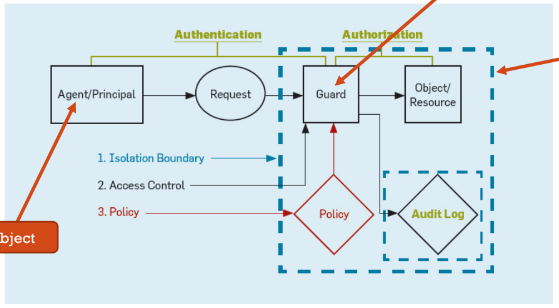
\includegraphics[scale=0.5]{06/AccessControSchema.png}
        \caption{Schema di un sistema di controllo degli accessi}
    \end{figure}

    Dallo schema raffigurato possiamo denotare che:
    \begin{itemize}
        \item \textbf{Soggetto} (\textit{Agent/Principal}): è l'entità che vuole accedere ad un oggetto o una risorsa, questo deve essere autenticato e autorizzato per poter accedere. Ad esempio un operatore di cassa di una banca non può accedere ai dati dei clienti, ma dopo aver ricevuto opportuna autorizzazione può effettuare operazioni sui conti.
        \item \textbf{Richiesta} (\textit{Request}): è la richiesta di accesso fatta dal soggetto. Questa contiene diverse informazioni che vedremo in seguito.
        \item \textbf{Confine di Isolamento} (\textit{Isolation Boundary}): è il confine che separa il soggetto dal sistema che contiene l'oggetto o la risorsa. Questo confine è importante per garantire che il soggetto non possa accedere direttamente all'oggetto o alla risorsa.
        \item \textit\textbf{Guard} (\textit{Policy Decision Point}): è l'entità che decide se il soggetto può accedere all'oggetto o alla risorsa. Questo prende decisioni basandosi su regole di autorizzazione.  
        \item \textit\textbf{Policy}: è l'insieme di regole che il \textit{guard} deve seguire per decidere se il soggetto può accedere all'oggetto o alla risorsa.
        \item \textbf{Oggetto} (\textit{Object/Resource}): è l'entità a cui il soggetto vuole accedere. Questo può essere un file, un database, un dispositivo, ecc\dots Questo deve essere protetto per garantire la confidenzialità e l'integrità delle informazioni.
        \item \textbf{Sistema Controllo Accessi} (\textit{Access Control }): è il punto dove avviene il controllo degli accessi. (Solitamente il \textit{guard} è una parte di questo sistema).
        \item \textit\textbf{Audit Log}: è il registro che contiene tutte le informazioni riguardanti le richieste di accesso sia autorizzate che non autorizzate. Questo è importante per monitorare il sistema e per rilevare eventuali attacchi.
    \end{itemize}
    
    \paragraph{Alcune note} Il confine di Isolamento tra il soggetto e tutto il resto del sistema è molto importante per garantire che nessuno possa accedere direttamente all'oggetto o alla risorsa senza passare per il \textit{guard}. Solo degli utenti con privilegi speciali, quali "amministratori" possono \textit{by-passare il guard} questo solo per aggiornare delle \textit{policy} o altri aggiornamenti al sistema. Infine è presente anche una \textit{inner boundary} che garantisce l'integrità dell'\textit{audit log}, questa non può essere \textit{by-passata} da nessuno, nemmeno dagli amministratori.
    \subsection{I Sistemi Operativi}
        I sistemi operativi sono esempi di sistemi che implementano il controllo degli accessi. Questi infatti non permettono di accedere direttamente alle risorse \textit{hardware} e \textit{software} del sistema, ma forniscono un'interfaccia per accedere a queste. Inoltre alcuni \texttt{SO} supportano multi-utente e multi-tasking, dove per il primo bisogna implementare un sistema per garantire accesso allo stesso tempo e/o in modo concorrente a più utenti, mentre per il secondo bisogna sviluppare un sistema per garantire che più processi in parallelo possano accedere alle risorse del sistema in modo concorrente.
        \subsubsection{Struttura del \texttt{SO}}
            Un sistema operativo è composto da una memoria, accessibile agli utenti, la quale comunica con il sistema operativo che tramite appositi meccanismi di controllo degli accessi permette di accedere al \texttt{I/O} \textit{bus} dove sono collocate le \texttt{I/O} \textit{interfaces} che permettono di accedere alle risorse del sistema (dischi, stampanti,\dots).\newline
            In questo sistema bisogna proteggere la memoria, i file contenuti nei dischi, controllare l'accesso degli utenti tramite meccanismi di autenticazione e autorizzazione e infine proteggere in generale il controllo degli accessi.
            \paragraph{Cosa implementa \texttt{SO}} Facendo riferimento alla figura \figref{fig:accessControlSchema}, il sistema operativo dunque implementa l'autenticazione, l'autorizzazione e la barriera di isolamento esterna per garantire che le \textit{policy} siano rispettate.
    \subsection{Definizione, Scopo e \textit{Policy} di un \texttt{AC}}
        \paragraph{Definizione} Un sistema di controllo accessi è definito come il processo che \textbf{media} le \textbf{richieste} alle risorse e ai dati di un sistema determinando se la richiesta di accesso deve essere approvata o rifiutata.
            \subparagraph{\textit{Flow} della richiesta} \begin{enumerate}
                \item Una richiesta di accesso $(s,a,r)$ viene fatta da un soggetto $s$ per accedere ad un oggetto $r$ tramite un'azione $a$. Questa arriva al modulo di controllo accessi
                \item Il modulo di controllo accessi prende la decisione se approvare (\textit{grant}) o rifiutare (\textit{deny}) la richiesta.
                \item Se la risposta è \textit{grant} allora $s$ può eseguire l'operazione $a$ su $r$, altrimenti se la risposta è \textit{deny} allora $s$ è informato che \underline{non} può eseguire l'operazione $a$ su $r$.
            \end{enumerate}
        Questo processo è di fondamentale importanza in un qualsiasi sistema di sicurezza.